%!TEX root = ../thesis.tex

%%%%% Chapter: System Evaluation %%%%%
\chapter{Evaluation Framework}

\ifpdf
    \graphicspath{{Chapter7/Figs/Raster/}{Chapter7/Figs/PDF/}{Chapter7/Figs/}}
\else
    \graphicspath{{Chapter7/Figs/Vector/}{Chapter7/Figs/}}
\fi


\section{Overview}

\section{The Ground-Truth Data}

The ground-truth data of a single set of input lecture data (a handout PDF file + its associated audio file) can be seen as the correct mappings from the handout chunks (\texttt{BBoxGroup} objects) to the corresponding parts of the audio file (\texttt{TIntervalGroup} objects). The ground truth data as a whole can be represented by a \texttt{Matches} object described in \Cref{sec:basic-elem-matches}.

The ground-truth data should be labelled at the finest spatial scale possible, which means each \texttt{BBoxGroup} object in the ground-truth data is supposed to be as small (in its total area) as possible. This ensures the feasibility of the multi-scale evaluation of the alignment algorithm.

\section{Evaluating the Tesseract PLA}

Recall that the page layout analysis (PLA) of the Tesseract OCR engine produces a set of bounding-boxes which identifies distinct text regions in the PDF input. In \Cref{fig:eval-ocr-pla}, we can see how true positives (TP), true negatives (TN), false positives (FP) and false negatives (FN) are identified, given the bounding-boxes (a \texttt{BBoxGroups} object as a whole) in the ground-truth data. Here we assume that the bounding-boxes are non-overlapping for the ground-truth data and the OCR output respectively (in practice the OCR output bounding-boxes may overlap a little bit).

\begin{figure}[!htb]
    \centering
    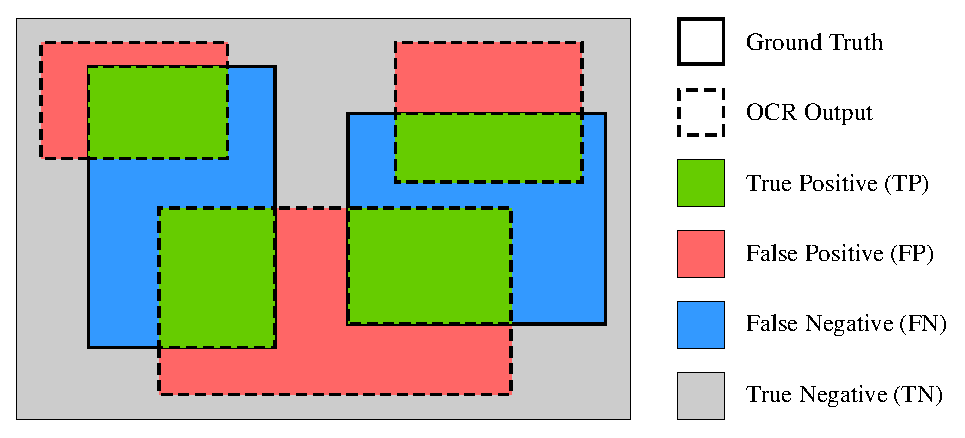
\includegraphics[width=0.75\textwidth]{eval-ocr-pla.eps}
    \caption{TP, TN, FP and FN in the evaluation of PLA}
    \label{fig:eval-ocr-pla}
\end{figure}

The key evaluation metrics are the \textit{true positive rate} (TPR) and \textit{true negative rate} (TNR), which are calculated as follows:
\[
    \begin{cases}
        \text{TPR \,=\, TP / (TP + FN)} \\
        \text{TNR =\, TN / (TN + FP)}
    \end{cases}
\]
Note that TPR is also called the recall rate. To calculate TPR and TNR, we sum up all rectangle areas for each certain type (TP, TN, FP and FN) and then substitute the values into the above equations.

The TPR (recall rate) essentially measures the fraction of the intersection area between the OCR output bounding-boxes and the bounding-boxes of the ground-truth data, with respect to the total area of the ground-truth bounding-boxes. The TNR, on the other hand, reflects how much useless area is included in the OCR output. Clearly we should maximise the TPR and minimise the TNR.


\section{Evaluating the OCR Text Recognition}

The text recognition accuracy of the Tesseract OCR engine is measured by the \textit{word error rate} (WER). Let $X$ be the concatenation of all words in the OCR recognition result (a \texttt{BBoxGroups} object) and let $Y$ be the concatenation of all words in the \texttt{BBoxGroup} objects of the ground-truth data (recall that the ground-truth data as a whole is a \texttt{Matches} object). We first obtain the optimal alignment $Z_{opt}$ of $X$ and $Y$ using the following joint weight function:
\begin{equation}
    \mathcal{F}(x,y) = 
    \begin{cases}
        0 & x = y \text{ (match)} \\
        -4 & x = \phi \text{ (insertion) or } y = \phi \text{ (deletion)} \\
        -6 & x \neq y \neq \phi \text{ (substitution)}
    \end{cases}
\end{equation}
The weight ratio of insertion, deletion and substitution is defined as 4:4:6 since we want a single substitution to cost more than a single insertion or substitution, but cost less than an insertion plus a substitution. 

Let $I$, $D$ and $S$ be the numbers of insertions, deletions and substitutions in the optimal alignment $Z_{opt}$. Then the WER of OCR text recognition is calculates as:
\begin{equation}
    \text{WER} = \frac{I + D + S}{N}
\end{equation}
where $N$ is the length of the reference string $Y$ (ground-truth).


\section{Evaluating the Alignment Algorithm}

Evaluation of the alignment algorithm is more difficult since the scale of the OCR output bounding-boxes (a \texttt{BBoxGroups} object as a whole) may vary. We first need to find the correct ground-truth audio segments (\texttt{TIntervalGroup} object) for each bounding-box (at different scales) of the OCR output, and then compare the segments from the output of the alignment algorithm with the correct segments. 

\subsection{Dealing with Multiple Scales}

Let's start with an example. \Cref{fig:eval-align-scale} shows 3 different OCR output bounding-boxes of various scales (in 3 different colors other than black) and their assigned ground-truth audio segments. The ground-truth bounding-boxes (\texttt{BBoxGroup} objects) and their matching audio segments (\texttt{TIntervalGroup} objects) are shown in black. 

\begin{figure}[!tb]
    \centering
    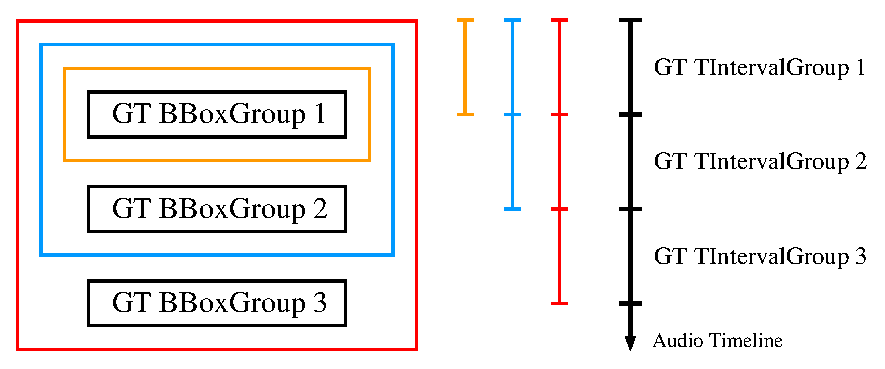
\includegraphics[width=.8\textwidth]{eval-align-scale.eps}
    \caption{Relationship between the scale of the bounding-box and its assigned ground-truth audio segments}
    \label{fig:eval-align-scale}
\end{figure}

It's clear that the number of assigned ground-truth audio segments generally increases with the bounding-box scale. For example in \Cref{fig:eval-align-scale}, the yellow bounding-box encloses only the first \texttt{BBoxGroup} object and is assigned just the first ground-truth audio segment, while the red bounding-box includes all the \texttt{BBoxGroup} objects so it is assigned all three audio segments.

